\documentclass[tikz,border=12pt]{standalone}
\usepackage[T1]{fontenc}
\usepackage{tgheros}
\usepackage{sfmath}
\usepackage{amsmath}
\usepackage{fontawesome5}
\usepackage{tikz}
\usetikzlibrary{arrows.meta,positioning,shapes.geometric,fit,backgrounds,calc}
\usepackage{xcolor}

\renewcommand{\familydefault}{\sfdefault}

% Semantic Palette from visual-system.md
\definecolor{navy}{HTML}{1B2A4A}
\definecolor{navylight}{HTML}{E8EDF6}
\definecolor{teal}{HTML}{168F84}
\definecolor{teallight}{HTML}{E4F6F3}
\definecolor{amber}{HTML}{C98218}
\definecolor{amberlight}{HTML}{FFF3DC}
\definecolor{coral}{HTML}{BD4F2F}
\definecolor{corallight}{HTML}{FAE9E2}
\definecolor{violet}{HTML}{6550A8}
\definecolor{violetlight}{HTML}{F0ECFA}
\definecolor{slate}{HTML}{687386}
\definecolor{slatelight}{HTML}{F4F6F7}
\definecolor{cardborder}{HTML}{CBD5E1}

\begin{document}
\begin{tikzpicture}[
  font=\sffamily,
  >=Stealth,
  statecard/.style={
    draw=cardborder,
    fill=white,
    rounded corners=5pt,
    line width=1.1pt,
    inner sep=8pt,
    minimum height=1.95in,
    align=center,
    text=navy
  },
  manualcard/.style={
    draw=violet,
    fill=violetlight,
    rounded corners=5pt,
    line width=1.3pt,
    inner sep=8pt,
    minimum height=1.95in,
    align=center,
    text=navy
  },
  autoncard/.style={
    draw=teal,
    fill=teallight,
    rounded corners=5pt,
    line width=1.3pt,
    inner sep=8pt,
    minimum height=1.95in,
    align=center,
    text=navy
  },
  sharedcard/.style={
    draw=amber,
    fill=amberlight,
    rounded corners=5pt,
    line width=1.3pt,
    inner sep=8pt,
    minimum height=1.95in,
    align=center,
    text=navy
  },
  estopcard/.style={
    draw=coral,
    fill=corallight,
    rounded corners=5pt,
    line width=1.4pt,
    inner sep=8pt,
    align=center,
    text=coral
  },
  transarrow/.style={
    ->,
    line width=1.1pt,
    draw=navy!80
  },
  estoparrow/.style={
    ->,
    line width=1.3pt,
    draw=coral
  },
  badgelabel/.style={
    font=\sffamily\scriptsize\bfseries,
    fill=white,
    draw=cardborder,
    rounded corners=3pt,
    inner sep=2.5pt,
    align=center,
    text=navy
  }
]

  % Title banner / Authority Hierarchy
  \node[draw=navy!30, fill=slatelight, rounded corners=4pt, line width=0.8pt, text width=7.6in, align=center, inner sep=6pt] (topbanner) {
    \textbf{\faIcon{balance-scale}\; DETERMINISTIC HUMAN--MACHINE AUTHORITY HIERARCHY}\\[2pt]
    {\footnotesize \textbf{P0:} Zero-Software Hardware E-Stop \quad$>$\quad \textbf{P1:} Manual Preemption \quad$>$\quad \textbf{P2:} MCU Safety Filter \quad$>$\quad \textbf{P3:} MPU Neural Proposal}
  };

  % Row 1: The Three Operational States
  % State 1: MANUAL TELEOPERATION
  \node[manualcard, text width=2.25in, below=1.20in of topbanner.south west, anchor=north west] (manual) {
    \textbf{\color{violet}\faIcon{gamepad}\; 1. MANUAL OVERRIDE}\\[3pt]
    {\footnotesize \textbf{Primary Authority:} Human Operator}\\
    {\scriptsize Direct pendant / joystick MCU stream}\\[5pt]
    \rule{2.0in}{0.4pt}\\[5pt]
    \begin{minipage}{2.1in}
    \scriptsize
    $\bullet$ Neural proposals disabled\\
    $\bullet$ Bumpless tracking integrator sync\\
    $\bullet$ Real-time kinematic limits clamped
    \end{minipage}
  };

  % State 2: SHARED / COOPERATIVE
  \node[sharedcard, text width=2.25in, right=0.42in of manual] (shared) {
    \textbf{\color{amber}\faIcon{hands-helping}\; 2. SHARED CONTROL}\\[3pt]
    {\footnotesize \textbf{Blended Authority:} Human + Policy}\\
    {\scriptsize Dynamic torque blending / admittance}\\[5pt]
    \rule{2.0in}{0.4pt}\\[5pt]
    \begin{minipage}{2.1in}
    \scriptsize
    $\bullet$ $\mathbf{u}(t) = \alpha(t)\mathbf{u}_{\text{h}} + (1-\alpha(t))\mathbf{u}_{\text{p}}$\\
    $\bullet$ $\mathcal{C}^2$ quintic smoothstep ramp\\
    $\bullet$ Jerk-bounded acceleration clamp
    \end{minipage}
  };

  % State 3: FULLY AUTONOMOUS
  \node[autoncard, text width=2.25in, right=0.42in of shared] (auton) {
    \textbf{\color{teal}\faIcon{robot}\; 3. AUTONOMOUS LEASE}\\[3pt]
    {\footnotesize \textbf{Governed Authority:} Neural MPU}\\
    {\scriptsize 20 Hz Diffusion/ACT action chunks}\\[5pt]
    \rule{2.0in}{0.4pt}\\[5pt]
    \begin{minipage}{2.1in}
    \scriptsize
    $\bullet$ Active dead-man consent lease\\
    $\bullet$ 1000 Hz MCU barrier verification\\
    $\bullet$ Truncated episode telemetry tag
    \end{minipage}
  };

  % Direct Preemption from Auton to Manual (Positioned in the gap between banner and cards)
  \draw[transarrow, line width=1.4pt, draw=violet] ($(auton.north)!0.5!(auton.north west)$) to[out=140, in=40] 
    node[pos=0.5, above, badgelabel, draw=violet!60] {\faIcon{hand-paper}\; \textbf{Immediate Preemptive Takeover} ($\|\mathbf{u}_{\text{human}}\| > \delta_{\text{takeover}}$)} ($(manual.north)!0.5!(manual.north east)$);

  % Row 2: EMERGENCY STOP STATE (Centered below)
  \node[estopcard, text width=7.6in, below=0.55in of shared.south] (estop) {
    \textbf{\color{coral}\faIcon{exclamation-triangle}\; CATEGORY 0 / 1 EMERGENCY STOP (ZERO-SOFTWARE HARDWARE INTERLOCK)}\\[3pt]
    {\footnotesize \textbf{Ultimate Physical State:} Actuator Coils De-Energized $\cdot$ Dynamic Injection Braking $\cdot$ Mechanical Spring Brakes Locked}\\
    {\scriptsize Triggered by: Physical E-stop Button Pressed $\cdot$ MCU Hardware Watchdog Timeout $\cdot$ CBF Safety Barrier Hard Violation $\cdot$ Driver Overcurrent}
  };

  % Horizontal Transitions between Manual, Shared, Auton
  \draw[transarrow] ($(manual.east)+(0,0.35in)$) -- ($(shared.west)+(0,0.35in)$)
    node[pos=0.5, above, badgelabel] {Arm / Engage\\{\scriptsize Blending ramp}};

  \draw[transarrow] ($(shared.west)-(0,0.35in)$) -- ($(manual.east)-(0,0.35in)$)
    node[pos=0.5, below, badgelabel] {Seize Control\\{\scriptsize $\|\mathbf{u}_{\text{h}}\| > \delta_{\text{takeover}}$}};

  \draw[transarrow] ($(shared.east)+(0,0.35in)$) -- ($(auton.west)+(0,0.35in)$)
    node[pos=0.5, above, badgelabel] {Consent Granted\\{\scriptsize $\alpha(t) \to 0$}};

  \draw[transarrow] ($(auton.west)-(0,0.35in)$) -- ($(shared.east)-(0,0.35in)$)
    node[pos=0.5, below, badgelabel] {Intervention Detected\\{\scriptsize Bumpless filter $\alpha \uparrow$}};

  % Transitions down to E-Stop
  \draw[estoparrow] (manual.south) -- (manual.south |- estop.north)
    node[pos=0.5, fill=white, inner sep=2pt, font=\sffamily\scriptsize\bfseries, text=coral] {Physical E-Stop};

  \draw[estoparrow] (shared.south) -- (estop.north)
    node[pos=0.5, fill=white, inner sep=2pt, font=\sffamily\scriptsize\bfseries, text=coral] {Watchdog / Safety Trip};

  \draw[estoparrow] (auton.south) -- (auton.south |- estop.north)
    node[pos=0.5, fill=white, inner sep=2pt, font=\sffamily\scriptsize\bfseries, text=coral] {Lease Expired / Veto Trip};

  % Reset recovery path from E-Stop back to Manual
  \draw[transarrow, dashed, draw=slate] (estop.west) -- ++(-0.28in, 0) |- 
    node[pos=0.25, left, font=\sffamily\scriptsize\bfseries, text=slate, align=center] {Physical Key Reset\\+ Operator Acknowledge} (manual.west);

\end{tikzpicture}
\end{document}
